\chapter{Implementation of the \nameref*{sec:design:riot_registry}}
\label{chapter:implementation}

This chapter shows the implementation details of \autoref{chapter:design}.
The full source code is on the enclosed CD and on GitHub \footnote{\url{https://github.com/LasseRosenow/riot-runtime-config}}.

\section{\glsfirst*{ac:cs}}

This section shows the implementation details of the in \autoref{sec:design:riot_registry:configuration_schemas} specified \glspl{ac:cs}.
The ``sys''-\gls{ac:cn} \glspl{ac:cs} are implemented in an additional module called ``registry\_schemas''.
By default every \gls{ac:cs}, that is implemented inside that module is disabled, because those implementations are depending on CFLAGS to be set.
The structure of those CFLAGS is the following:
``DCONFIG\_REGISTRY\_ENABLE\_SCHEMA\_\{schema\_name\}'', where ``{schema\_name\}'' must be replaced with the name of an existing \gls{ac:cs} such as ``RGB\_LED'' or ``FULL\_EXAMPLE''.

\autoref{fig:riot_registry_schema_structure} shows the structure of a \gls{ac:cs}.
It consists of an id, which is used in the \gls{ac:cp}, a name and description metadata field so that \glspl{gl:configuration_manager} can provide a less confusing interface, a list of \glspl{ac:si} and an items field, which contains an array of ``Schema Items''.
The list of \glspl{ac:si} needs to be stored in the \gls{ac:cs} because the \nameref{sec:design:riot_registry} is supposed to do avoid dynamic heap allocation (see \autoref{sec:requirements:binary_internal_configuration_parameter_format}). This list is a linked list, so every newly registered \gls{ac:si} will be added at the end of the list.
The Schema Items of the items field represent either a configuration parameter or a \gls{ac:cg}. Each Schema Item has a Registry ID as well as a name and a description metadata field. If a Schema Item is a \gls{ac:cg}, then it contains an array of Schema items as its value union field. Otherwise it contains a configuration parameter type of the concrete type ``Registry Type''.

Besides its fields the \gls{ac:cs} also contains a callback function inside its ``mapping'' field.
This function translates a configuration parameter ID to a pointer of the configuration parameter's value inside the \gls{ac:si}.
It also returns the size of this configuration parameter value.
This function is necessary because how a \gls{ac:si} stores its data is decided by each \gls{ac:cs}'s implementation. So only the \gls{ac:cs} knows how to translate between a configuration parameter ID and the actual data location inside the \gls{ac:si}.

\begin{figure}[H]
    \centering
    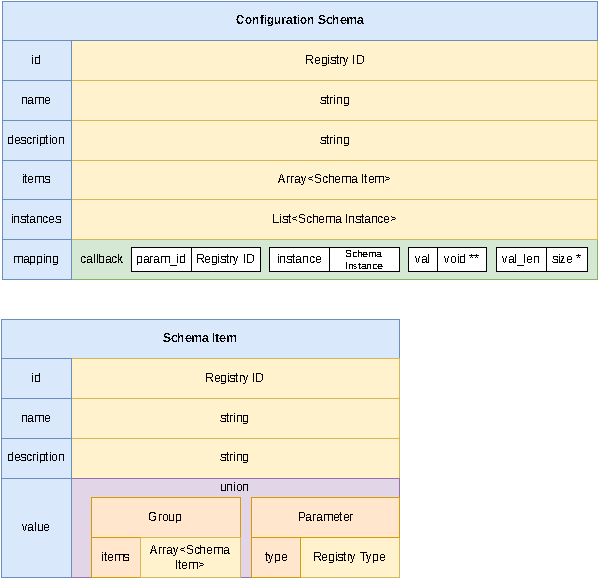
\includegraphics[width=\textwidth]{data_structure_schema}
    \caption{\nameref{sec:design:riot_registry} \gls{ac:cs} implementation data structure.}
    \label{fig:riot_registry_schema_structure}
\end{figure}

\autoref{fig:riot_registry_configuration_parameter_type_enum} shows the data structure of the ``Registry Type'' type.
A Registry Type is an enum that can be either of type ``none'', if the type is not known.
This is usually used to show, that something went wrong or as a placeholder for as long as a type is not yet known.
It can also have the type ``opaque''.
This is used to allow the \nameref{sec:design:riot_registry} to support every other type of data that does not fit into one of the other types.
It internally has the void pointer type and a specified size.
Additionally a string of a fixed size, a boolean, a uint8, a uint16, a uint32, a uint64, a int8, a int16, a int32, a int64, a float32 and a float64 are supported as a Registry Type.

\begin{figure}[H]
    \centering
    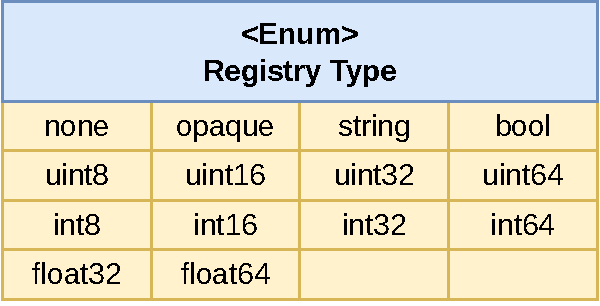
\includegraphics[width=0.5\textwidth]{data_structure_registry_type}
    \caption{\nameref{sec:design:riot_registry} configuration parameter type implementation enum.}
    \label{fig:riot_registry_configuration_parameter_type_enum}
\end{figure}

\autoref{fig:riot_registry_schema_instance_structure} shows the data structure of a \gls{ac:si}.
The ``name'' field allows it \gls{ac:si} to have a human readable soft identifier.
The ``data'' field contains its configuration parameter values in whatever format the \gls{ac:cs} implementation decides on.
The ``commit\_cb'' callback function is called whenever a configuration parameter's new value of this \gls{ac:si} gets ``committed'' (see \autoref{sec:design:commit_configurations}).
This way the module or driver that holds this \gls{ac:si} can apply the configuration parameter changes inside the ``commit\_cb'' function.


\begin{figure}[H]
    \centering
    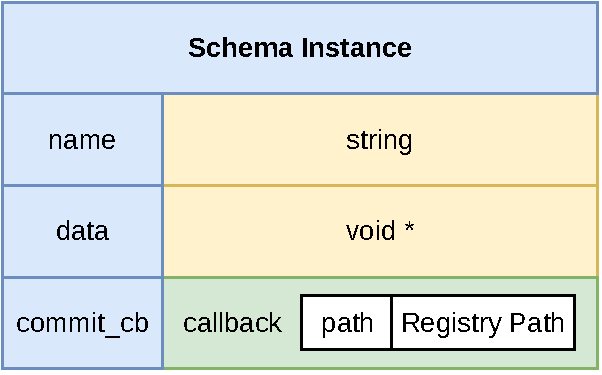
\includegraphics[width=0.5\textwidth]{data_structure_schema_instance}
    \caption{\nameref{sec:design:riot_registry} \gls{ac:si} implementation data structure.}
    \label{fig:riot_registry_schema_instance_structure}
\end{figure}

\autoref{lst:registry_schemas_h} shows the header file of the ``registry\_schemas'' module with an example RGB LED \gls{ac:cs}.
In line 4 the ``registry\_schema\_init'' function is defined, which registers all enabled ``sys''-\gls{ac:cn} \glspl{ac:cs} at the \nameref{sec:design:riot_registry}.
From line 7 - 10 is an enum that defines which \gls{ac:cs} gets which ID.
This enum prevents that two \glspl{ac:cs} use the same ID.
In line 13 the \gls{ac:cs} variable is created which will be implemented in the corresponding C file.
Line 16 - 21 is the struct definition of a \gls{ac:si}. For a RGB LED \gls{ac:cs} a red, green and blue uint8 value is enough.
In line 24 - 28 the configuration parameter IDs are set using an enum again.
These will be used in the C file, when implementing the \gls{ac:cs}.

\begin{lstlisting}[
    language=c,
    caption={Example \gls{ac:cs} implementation: registry\_schemas.h},
    label={lst:registry_schemas_h}
]
#include "registry.h"

/* initialize schemas */
void registry_schemas_init(void);

/* schema IDs */
typedef enum {
    REGISTRY_SCHEMA_RGB_LED      = 1,
    /* SOME_OTHER_SCHEMA         = 2, ... */
} registry_schema_id_t;

/* RGB LED schema */
extern registry_schema_t registry_schema_rgb_led;

/* RGB LED instance */
typedef struct {
    clist_node_t node;
    uint8_t red;
    uint8_t green;
    uint8_t blue;
} registry_schema_rgb_led_t;

/* RGB LED configuration parameter IDs */
typedef enum {
    REGISTRY_SCHEMA_RGB_LED_RED,
    REGISTRY_SCHEMA_RGB_LED_GREEN,
    REGISTRY_SCHEMA_RGB_LED_BLUE,
} registry_schema_rgb_led_indices_t;
\end{lstlisting}

\autoref{lst:registry_schemas_init_c} shows the source code of the ``registry\_schema\_init.c'' file.
In this C file, the ``registry\_schemas\_init'' function is implemented.
In line 6 it is checked if the ``CONFIG\_REGISTRY\_ENABLE\_SCHEMA\_RGB\_LED'' flag to enable the RGB LED \gls{ac:cs} is set.
If the flag is set, then in line 7 - 10 the RGB LED \gls{ac:cs} gets registered in the \nameref{sec:design:riot_registry}.
As the RGB LED schema is supposed to be a ``sys''-\gls{ac:cn} \gls{ac:cs}, the \gls{ac:cn} is set to 0 using the ``REGISTRY\_ROOT\_GROUP\_SYS'' enum value.
In line 9 the in \autoref{lst:registry_schemas_h} defined \gls{ac:cs} variable is passed as an argument.

\begin{lstlisting}[
    language=c,
    caption={Example \gls{ac:cs} implementation: registry\_schemas\_init.c},
    label={lst:registry_schemas_init_c}
]
#include "registry.h"
#include "registry_schemas.h"

void registry_schemas_init(void)
{
    if (IS_ACTIVE(CONFIG_REGISTRY_ENABLE_SCHEMA_RGB_LED)) {
        registry_register_schema(
            REGISTRY_ROOT_GROUP_SYS,
            &registry_schema_rgb_led,
        );
    }
}
\end{lstlisting}

\autoref{lst:registry_schema_rgb_led_c} shows the source code of the ``registry\_schema\_rgb\_led.c'' file. It contains an example RGB LED \gls{ac:cs} implementation.
To create a \gls{ac:cs}, the ``REGISTRY\_SCHEMA'' macro can be used as seen in line 3.
This macro takes the in \autoref{lst:registry_schemas_h} defined \gls{ac:cs} variable, the \gls{ac:cs} ID, 2 strings and a ``mapping'' function as its arguments.
Additionally as can be seen from line 9 - 19, it can take infinitely more configuration parameter macros (``REGISTRY\_PARAMETER\_*'') or \gls{ac:cg} macros (``REGISTRY\_GROUP'') as its arguments. The latter not being present in this example.
With these values, the macros generate a struct of the structure explained in \autoref{fig:riot_registry_schema_structure}.
In line 6 as an example, the first string will be the value of the name field and the second string will be the value of the description filed of the \gls{ac:cs} struct.
Line 23 to line 47 show the ``mapping'' function implementation.
In line 29 this function casts the data field of the \gls{ac:si} to the correct struct of this \gls{ac:cs}'s implementation.
From line 31 to 46, depending on which configuration parameter ID is provided, the output pointer of a pointer (``val'') gets set to the pointer of the \gls{ac:si}'s value. An example of this can be seen in line 33. The second output pointer's value (``val\_len'') gets set to the size of the configuration parameter's value. An example of this can be seen in line 34.

\begin{lstlisting}[
    language=c,
    caption={Example \gls{ac:cs} implementation: registry\_schema\_rgb\_led.c},
    label={lst:registry_schema_rgb_led_c}
]
#include "registry_schemas.h"

REGISTRY_SCHEMA(
    registry_schema_rgb_led,
    REGISTRY_SCHEMA_RGB_LED,
    "rgb", "Representation of an rgb color.",
    mapping,

    REGISTRY_PARAMETER_UINT8(
        REGISTRY_SCHEMA_RGB_LED_RED,
        "red", "Intensity of the red color of the rgb lamp.")

    REGISTRY_PARAMETER_UINT8(
        REGISTRY_SCHEMA_RGB_LED_GREEN,
        "green", "Intensity of the green color of the rgb lamp.")

    REGISTRY_PARAMETER_UINT8(
        REGISTRY_SCHEMA_RGB_LED_BLUE,
        "blue", "Intensity of the blue color of the rgb lamp.")

    );

static void mapping(
    const registry_id_t param_id,
    const registry_instance_t *instance,
    void **val,
    size_t *val_len,
) {
    registry_schema_rgb_led_t *_instance = (registry_schema_rgb_led_t *)instance->data;

    switch (param_id) {
    case REGISTRY_SCHEMA_RGB_LED_RED:
        *val = &_instance->red;
        *val_len = sizeof(_instance->red);
        break;

    case REGISTRY_SCHEMA_RGB_LED_GREEN:
        *val = &_instance->green;
        *val_len = sizeof(_instance->green);
        break;

    case REGISTRY_SCHEMA_RGB_LED_BLUE:
        *val = &_instance->blue;
        *val_len = sizeof(_instance->blue);
        break;
    }
}
\end{lstlisting}

\autoref{lst:example_cs_main_c} shows an example application that uses the RGB LED \gls{ac:cs}.
From line 5 - 25 the \gls{ac:si} callback function is implemented.
In this implementation this function only prints the \gls{ac:cn}, \gls{ac:cs} and \gls{ac:si} of the committed \gls{ac:cp}, if the \gls{ac:cp} parameter ``path'' provides these values.
From line 28 - 32 a variable that initializes an RGB LED \gls{ac:si} struct, giving default values to the red, green and blue fields.
From line 35 - 39 a variable is defined, initializing a \nameref{sec:design:riot_registry} \gls{ac:si} struct.
This struct takes the callback function of line 5 and the RGB LED \gls{ac:si} struct as its value.
In line 44 the registry gets initialized by calling the ``registry\_init'' function.
Then in line 47 the \glspl{ac:cs} get initialized by calling the ``registry\_schemas\_init'' function. And finally from line 50 - 54 the \nameref{sec:design:riot_registry} \gls{ac:si} struct that got initialized in line 35, is registered in the \nameref{sec:design:riot_registry} using the ``registry\_register\_schema\_instance'' function, providing the ``sys'' \gls{ac:cn} and the id of the \gls{ac:cs} as additional arguments.

\begin{lstlisting}[
    language=c,
    caption={Example \gls{ac:cs} implementation: main.c},
    label={lst:example_cs_main_c}
]
#include "registry.h"
#include "registry_schemas.h"

/* schema instance commit callback */
int rgb_led_instance_0_commit_cb(
    const registry_path_t path,
    const void *context,
) {
    (void)context;

    /* print CN, CS ID and SI ID if available */
    printf("RGB instance commit_cb was executed: %d", *path.namespace_id);
    
    if (path.schema_id) {
        printf("/%d", *path.schema_id);
    }

    if (path.instance_id) {
        printf("/%d", *path.instance_id);
    }
    
    printf("\n");
    
    return 0;
}

/* schema instance data struct */
registry_schema_rgb_led_t rgb_led_instance_0_data = {
    .red = 0,
    .green = 255,
    .blue = 70,
};

/* schema instance */
registry_instance_t rgb_led_instance_0 = {
    .name = "rgb-0",
    .data = &rgb_led_instance_0_data,
    .commit_cb = &rgb_led_instance_0_commit_cb,
};

int main(void)
{
    /* init registry */
    registry_init();

    /* init schemas */
    registry_schemas_init();

    /* register schema instance */
    registry_register_schema_instance(
        REGISTRY_NAMESPACE_SYS,
        registry_schema_rgb_led.id,
        &rgb_led_instance_0,
    );

    return 0;
}
\end{lstlisting}

\section{\glsfirst*{ac:sf}}

This section shows the implementation details of the in \autoref{sec:design:riot_registry:storage_facilities} specified \glspl{ac:sf}.
The \nameref{sec:design:riot_registry} comes with a few officially supported \glspl{ac:sf} implemented in the ``registry\_storage\_facilities'' module.
By default every \gls{ac:sf}, that is implemented inside that module is disabled, because those implementations are depending on CFLAGS to be set.
The structure of those CLFAGS is the following: ``DCONFIG\_REGISTRY\_ENABLE\_STORAGE\_FACILITY\_\{storage\_facility\_name\}”'', where ``\{storage\_facility\_name\}'' must be replaced with the name of an existing \gls{ac:sf} such as ``VFS''.

\autoref{fig:riot_registry_storage_facility_structure} shows the structure of a \gls{ac:sf}.
It consists of four callback functions.
A ``load'' callback function that both take a ``Storage Facility Instance'', a \gls{ac:cp} and another callback as its arguments.
Inside the load function the \gls{ac:sf} searches for configuration parameter values of the given \gls{ac:cp}.
Therefor it might need for example a filesystem mount.
This is specified in the data field of the ``Storage Facility Instance'' as a void pointer.
The callback argument of the load callback takes a \gls{ac:cp} and a ``Registry Value'' as an argument.
This callback gets executed on every configuration parameter that is found and matches the provided \gls{ac:cp}.
The \nameref{sec:design:riot_registry} sets this callback to the ``registry\_value\_set'' function.
Besides the ``load'' callback function, the \gls{ac:sf} struct also has a ``save\_start'' and a ``safe\_end'' callback function.
Both take the ``Storage Facility Instance'' as an argument.
The ``save\_start'' callback function gets called before the ``save'' callback function gets executed and is used to initialize the storage device, for example to mount a filesystem before multiple save operations are executed.
This way unnecessary overhead of continuously mounting and unmounting filesystems can be avoided.
The ``save\_end'' callback function gets called after the ``save'' function finished its execution and is used to teardown the storage device, for example unmount a filesystem, after all ``save'' operations are completed.
The ``save'' callback function takes a ``Storage Facility Instance'', a \gls{ac:cp} and a ``Registry Value'' as its arguments.
It saves the provided configuration parameter value (Registry Value) on the storage, in a by the \gls{ac:sf} defined structure, so that the ``load'' function can find it by its \gls{ac:cp}.

\begin{figure}[H]
    \centering
    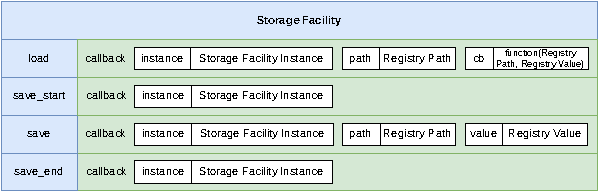
\includegraphics[width=\textwidth]{data_structure_storage_facility}
    \caption{\nameref{sec:design:riot_registry} \gls{ac:sf} implementation data structure.}
    \label{fig:riot_registry_storage_facility_structure}
\end{figure}

\autoref{fig:riot_registry_storage_facility_instance_structure} shows the structure of a \gls{ac:sf} Instance.
It holds a pointer to a \gls{ac:sf} implementation and provides data such as a filesystem mount as a void pointer.

\begin{figure}[H]
    \centering
    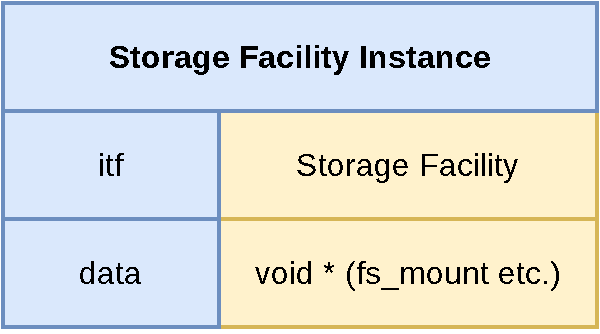
\includegraphics[width=0.44\textwidth]{data_structure_storage_facility_instance}
    \caption{\nameref{sec:design:riot_registry} \gls{ac:sf} Instance implementation data structure.}
    \label{fig:riot_registry_storage_facility_instance_structure}
\end{figure}

\autoref{fig:riot_registry_configuration_parameter_value} shows the structure of a configuration parameter called ``Registry Value''.
It has a ``type'' field which specifies the primitive type of the configuration parameter's value.
Its value is then stored in the ``buf'' field, which has a void pointer as its type.
To pass the buffer around the program safely, it is also important to know its size, so there is a third field with the name ``buf\_len'', which holds the size of the value, stored in the ``buf'' field.

\begin{figure}[H]
    \centering
    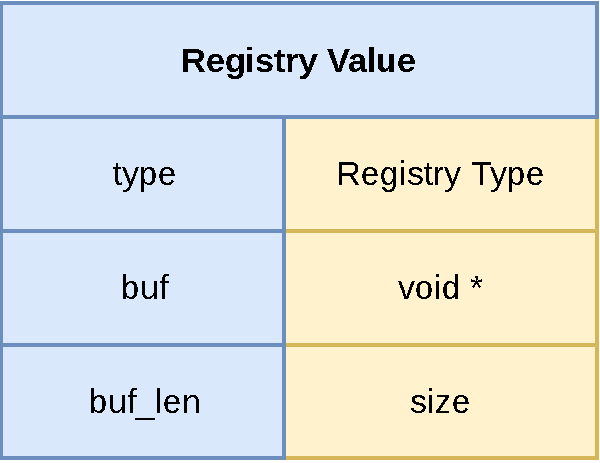
\includegraphics[width=0.4\textwidth]{data_structure_registry_value}
    \caption{\nameref{sec:design:riot_registry} configuration parameter value implementation structure.}
    \label{fig:riot_registry_configuration_parameter_value}
\end{figure}

\autoref{lst:registry_storage_facilities_h} shows the header file of the ``registry\_storage\_facilities'' module.
It contains an example ``VFS'' \gls{ac:sf} variable definition called ``registry\_storage\_facility\_vfs''.

\begin{lstlisting}[
    language=c,
    caption={Example \gls{ac:sf} implementation: registry\_storage\_facilities.h},
    label={lst:registry_storage_facilities_h}
]
#include "registry.h"

/* vfs storage facility instance */
extern registry_storage_facility_t registry_storage_facility_vfs;
\end{lstlisting}

\autoref{lst:registry_storage_facilitiy_vfs_c} shows the implementation of the VFS \gls{ac:sf}.
Because the full VFS \gls{ac:sf} implementation is around 400 lines of code, the provided \gls{ac:sf} source code in this thesis is reduced.
The full source code is on the enclosed CD and on GitHub \footnote{\url{https://github.com/LasseRosenow/riot-runtime-config/blob/main/external_modules/registry_storage_facilities/storage_facility_vfs.c}}.
In line 23 - 26 the \gls{ac:sf} variable is initialized and the load and save callback functions are taken as arguments.
The ``save'' function of the VFS \gls{ac:sf} creates a folder for every \gls{ac:cn} if it does not exist yet. It also creates a folder for every \gls{ac:cs} ID inside its \gls{ac:cn} folder. The same goes for the \gls{ac:si} ID, and the \gls{ac:cg} IDs. For the configuration parameters it does not create a folder, but create a file that also uses its ID as its filename.
Inside the file the configuration parameters value is written as binary.
The ``load'' function of the VFS \gls{ac:sf} scans the storage for folders and files that match the provided \gls{ac:cp}.
If those files match the \gls{ac:cp}, it asks the \nameref{sec:design:riot_registry} for the metadata of the configuration parameter by calling the ``registry\_get\_value'' function.
This way it can find out the correct size of the configuration parameters value and reads it from the storage.
This value is then returned using the provided callback function.

\begin{lstlisting}[
    language=c,
    caption={Example \gls{ac:sf} implementation: registry\_storage\_facility\_vfs.c},
    label={lst:registry_storage_facilitiy_vfs_c}
]
#include "registry_storage_facilities.h"

/* load data from storage */
static int load(
    const registry_storage_facility_instance_t *instance,
    const registry_path_t path,
    const load_cb_t cb,
    const void *cb_arg,
) {
    /* Loop through storage and call "load_cb_t" on each configuration parameter that is compatible to the specified path. */
}

/* save data to storage */
static int save(
    const registry_storage_facility_instance_t *instance,
    const registry_path_t path,
    const registry_value_t value
) {
    /* Open the file under the specified path and write the new value inside. */
}

/* storage facility */
registry_storage_facility_t registry_storage_facility_vfs = {
    .load = load,
    .save = save,
};
\end{lstlisting}

\autoref{lst:example_sf_main_c} shows the source code of an example application using the VFS \gls{ac:sf}.
From line 6 - 14 the filesystem mount is being configured.
Then in line 17 - 26 the VFS \gls{ac:sf} Instance is created, which takes the filesystem mount and the \gls{ac:sf} (``registry\_storage\_facility\_vfs'') as its field's values.
Then from line 28 - 38 the main function of the program is implemented.
First in line 31 the \nameref{sec:design:riot_registry} is initialized by calling the ``registry\_init'' function.
Then in line 34 the source \gls{ac:sf} is registered in the \nameref{sec:design:riot_registry} by calling the ``registry\_register\_storage\_facility\_src'' function. And finally in line 35 the destination \gls{ac:sf} is registered in the \nameref{sec:design:riot_registry} by calling the ``registry\_register\_storage\_facility\_dst'' function.

\begin{lstlisting}[
    language=c,
    caption={Example \gls{ac:sf} implementation: main.c},
    label={lst:example_sf_main_c}
]
#include "registry.h"
#include "registry_storage_facilities.h"
#include "fs/littlefs2_fs.h"

/* initialize vfs mount */
static littlefs2_desc_t fs_desc = {
    .lock = MUTEX_INIT,
};

static vfs_mount_t vfs_mount = {
    .fs = &FS_DRIVER,
    .mount_point = "/sda",
    .private_data = &fs_desc,
};

/* initialize a storage facility source instance */
registry_storage_facility_instance_t vfs_instance_src = {
    .itf = &registry_storage_facility_vfs,
    .data = &vfs_mount,
};

/* initialize a storage facility destination instance */
registry_storage_facility_instance_t vfs_instance = {
    .itf = &registry_storage_facility_vfs,
    .data = &vfs_mount,
};

int main(void)
{
    /* init registry */
    registry_init();

    /* register storage_facility source and destination instances */
    registry_register_storage_facility_src(&vfs_instance_src);
    registry_register_storage_facility_dst(&vfs_instance_dst);

    return 0;
}
\end{lstlisting}

\section{\glsfirst*{ac:cp}}

This section shows the implementation details of the in \autoref{sec:design:riot_registry:configuration_path} specified \gls{ac:cp}.

\autoref{fig:riot_registry_path_structure} shows the structure of the \gls{ac:cp} on the left-hand side.
It contains a \gls{ac:cn} field, that is implemented as an enum containing a ``sys''=0 and a ``app''=1 value as possible \glspl{ac:cn}.
The \gls{ac:cp} also has a \gls{ac:cs} ID field, which is of the type ``Registry ID''.
The Registry ID type internally is a uint32 type.
The \gls{ac:cp} also has a field that holds the \gls{ac:si} ID, which is also of the Registry ID type.
And at last the \gls{ac:cp} has a ``path'' field, which is an array of ``Registry IDs''.
The ``path'' field contains the \gls{ac:cg} and configuration parameter IDs.

\begin{figure}[H]
    \centering
    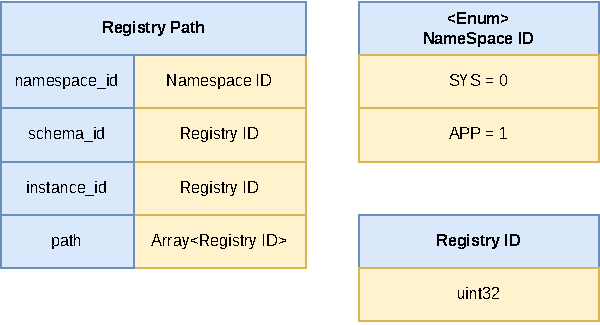
\includegraphics[width=0.8\textwidth]{data_structure_registry_path}
    \caption{\nameref{sec:design:riot_registry} \gls{ac:cp} implementation data structure.}
    \label{fig:riot_registry_path_structure}
\end{figure}

\section{\gls*{ac:api}}
\label{sec:implementation:riot_registry_api}

This section shows the implementation details of the in \autoref{sec:design:riot_registry:usage_flow} specified \gls{ac:api}.

\subsection{Basic \gls*{ac:api}}

\subsubsection{Get}

\autoref{fig:riot_registry_api_get} shows the implementation of how to get a configuration parameter's value as specified in \autoref{sec:design:riot_registry}.
It shows a function called ``get'' that takes a \gls{ac:cp} and a ``Registry Value'' pointer as an argument.
The ``Registry Value'' pointer is used to return the configuration parameter's value.

\begin{figure}[H]
    \centering
    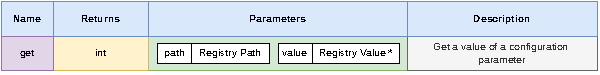
\includegraphics[width=\textwidth]{api_structure_get}
    \caption{\nameref{sec:design:riot_registry} \gls{ac:api}: get.}
    \label{fig:riot_registry_api_get}
\end{figure}

\autoref{lst:registry_get_function} shows the source code of this function.

\begin{lstlisting}[
    language=c,
    caption={Get configuration parameter values: C-function.},
    label={lst:registry_get_function},
]
int registry_get_value(
    const registry_path_t path,
    registry_value_t *value
);
\end{lstlisting}

\subsubsection{Set}

\autoref{fig:riot_registry_api_set} shows the implementation of how to set a configuration parameter's value to a new value as specified in \autoref{sec:design:riot_registry}.
It shows a function called ``set'' that takes a \gls{ac:cp} and a ``Registry Value'' as an argument.

\begin{figure}[H]
    \centering
    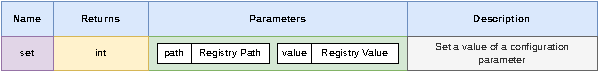
\includegraphics[width=\textwidth]{api_structure_set}
    \caption{\nameref{sec:design:riot_registry} \gls{ac:api}: set.}
    \label{fig:riot_registry_api_set}
\end{figure}

\autoref{lst:registry_set_function} shows the source code of this function.

\begin{lstlisting}[
    language=c,
    caption={Set new configuration parameter values: C-function.},
    label={lst:registry_set_function},
]
int registry_set_value(
    const registry_path_t path,
    const registry_value_t val
);
\end{lstlisting}

\subsubsection{Commit}

\autoref{fig:riot_registry_api_commit} shows the implementation of how to commit configuration parameters as specified in \autoref{sec:design:riot_registry}.
It shows a function called ``commit'' that takes a \gls{ac:cp} as an argument.

\begin{figure}[H]
    \centering
    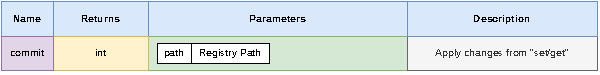
\includegraphics[width=\textwidth]{api_structure_commit}
    \caption{\nameref{sec:design:riot_registry} \gls{ac:api}: commit.}
    \label{fig:riot_registry_api_commit}
\end{figure}

\autoref{lst:registry_commit_function} shows the source code of this function.

\begin{lstlisting}[
    language=c,
    caption={Commit configuration parameters: C-function.},
    label={lst:registry_commit_function},
]
int registry_commit(const registry_path_t path);
\end{lstlisting}

\subsubsection{Export}

\autoref{fig:riot_registry_api_export} shows the implementation of how to export configuration parameters as specified in \autoref{sec:design:riot_registry}.
It shows a function called ``export'' that takes a \gls{ac:cp}, a callback function, a integer called ``recursion\_depth'' and a void pointer as for context data as an argument.
The ``recursion\_depth'' parameter of this function specifies how deep the export function is allowed to recursively search for configuration parameters and export them.
If the recursion\_depth is set to 0, then all configuration parameters, that are within the specified \gls{ac:cp} are exported.
If the recursion\_depth is set to 1, then only a configuration parameter gets exported, if it exactly matches the given \gls{ac:cp}.
If the recursion\_depth is set to a higher number than 1, the export function will export all configuration parameters, that are within the given \gls{ac:cp} and are not nested more steps deeper than the given \gls{ac:cp} goes plus the specified number.
The callback function takes a \gls{ac:cp}, a \gls{ac:cs}, a \gls{ac:si}, a ``Schema Item'' and a ``Registry Value'' and a void pointer for context data as its arguments.

\begin{figure}[H]
    \centering
    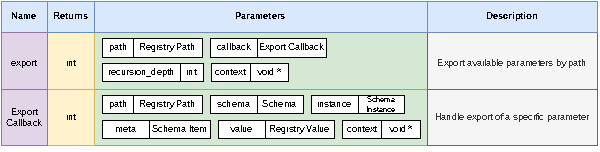
\includegraphics[width=\textwidth]{api_structure_export}
    \caption{\nameref{sec:design:riot_registry} \gls{ac:api}: export.}
    \label{fig:riot_registry_api_export}
\end{figure}

\autoref{lst:registry_export_function} shows the source code of this function.

\begin{lstlisting}[
    language=c,
    caption={Export configuration parameters: C-function.},
    label={lst:registry_export_function},
]
int registry_export(
    int (*export_func)(
        const registry_path_t path,
        const registry_schema_t *schema,
        const registry_instance_t *instance,
        const registry_schema_item_t *meta,
        const registry_value_t *value,
        const void *context
    ),
    const registry_path_t path,
    const int recursion_depth,
    const void *context,
);
\end{lstlisting}

\subsubsection{Load}

\autoref{fig:riot_registry_api_load} shows the implementation of how to load configuration parameter values from a non-volatile storage device as specified in \autoref{sec:design:riot_registry}.
It shows a function called ``load'' that takes a \gls{ac:cp} as an argument.

\begin{figure}[H]
    \centering
    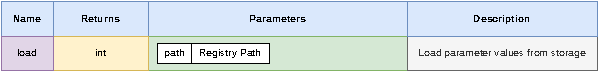
\includegraphics[width=\textwidth]{api_structure_load}
    \caption{\nameref{sec:design:riot_registry} \gls{ac:api}: load.}
    \label{fig:riot_registry_api_load}
\end{figure}

\autoref{lst:registry_load_function} shows the source code of this function.

\begin{lstlisting}[
    language=c,
    caption={Load configuration parameter values: C-function.},
    label={lst:registry_load_function},
]
int registry_load(const registry_path_t path);
\end{lstlisting}

\subsubsection{Save}

\autoref{fig:riot_registry_api_save} shows the implementation of how to save configuration parameter values to a non-volatile storage device as specified in \autoref{sec:design:riot_registry}.
It shows a function called ``save'' that takes a \gls{ac:cp} as an argument.

\begin{figure}[H]
    \centering
    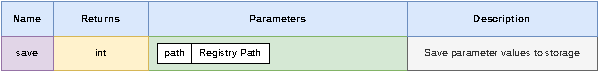
\includegraphics[width=\textwidth]{api_structure_save}
    \caption{\nameref{sec:design:riot_registry} \gls{ac:api}: save.}
    \label{fig:riot_registry_api_save}
\end{figure}

\autoref{lst:registry_save_function} shows the source code of this function.

\begin{lstlisting}[
    language=c,
    caption={Save configuration parameter values: C-function.},
    label={lst:registry_save_function},
]
int registry_save(const registry_path_t path);
\end{lstlisting}

\subsection{Schema Setup \gls*{ac:api}}

\autoref{fig:riot_registry_api_setup_schema} shows the implementation of how to register a \gls{ac:cs} or a \gls{ac:iot} in the \nameref{sec:design:riot_registry} as specified in \autoref{sec:design:riot_registry}.
It shows a function called ``register\_schema'' that takes a \gls{ac:cn} as an argument.
This function then adds the \gls{ac:cs} to a internal linked list.
\autoref{fig:riot_registry_api_setup_schema} also shows a function called ``register\_schema\_instance'', which takes a \gls{ac:cn}, a \gls{ac:cs} ID and a pointer to a \gls{ac:si} as its argument.
Internally the \nameref{sec:design:riot_registry} then adds the \gls{ac:si} to the linked list of \glspl{ac:si}, stored in the \gls{ac:cs} that matches the given \gls{ac:cs} ID.

\begin{figure}[H]
    \centering
    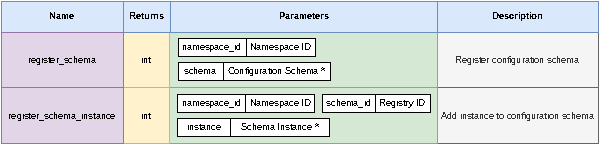
\includegraphics[width=\textwidth]{api_structure_setup_schema}
    \caption{\nameref{sec:design:riot_registry} \gls{ac:api}: setup \gls{ac:cs}.}
    \label{fig:riot_registry_api_setup_schema}
\end{figure}

\autoref{lst:registry_schema_setup_api} shows the source code of these functions.

\begin{lstlisting}[
    language=c,
    caption={Schema Setup \gls{ac:api}.},
    label={lst:registry_schema_setup_api},
]
void registry_schemas_init(void);

int registry_register_schema(
    const registry_namespace_id_t namespace_id,
    const registry_schema_t *schema
);

int registry_register_schema_instance(
    const registry_namespace_id_t namespace_id,
    const registry_id_t schema_id,
    const registry_instance_t *instance
);
\end{lstlisting}

\subsection{\acrlong*{ac:sf} Setup \gls*{ac:api}}

\autoref{fig:riot_registry_api_setup_storage_facility} shows the implementation of how to register a \gls{ac:sf} in the \nameref{sec:design:riot_registry} as specified in \autoref{sec:design:riot_registry}.
It shows a function called ``register\_storage\_facility\_src'' that takes a pointer to a \gls{ac:sf} Instance as an argument.
This function then adds the \gls{ac:sf} Instance to a internal linked list of \gls{ac:sf} sources.
\autoref{fig:riot_registry_api_setup_storage_facility} also shows a function called ``register\_storage\_facility\_dst'' that takes a pointer to a \gls{ac:sf} Instance as an argument.
This function then sets the \gls{ac:sf} Instance as the internal \gls{ac:sf}.
This \gls{ac:sf} is not added to a internal linked list, because there can only be one \gls{ac:sf} to write to.

\begin{figure}[H]
    \centering
    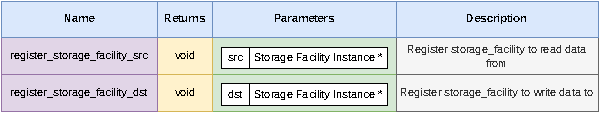
\includegraphics[width=\textwidth]{api_structure_setup_storage_facility}
    \caption{\nameref{sec:design:riot_registry} \gls{ac:api}: Setup \gls{ac:sf}.}
    \label{fig:riot_registry_api_setup_storage_facility}
\end{figure}

\autoref{lst:registry_storage_facility_setup_api} shows the source code of these functions.

\begin{lstlisting}[
    language=c,
    caption={\acrlong{ac:sf} Setup \gls{ac:api}.},
    label={lst:registry_storage_facility_setup_api},
]
void registry_register_storage_facility_src(
    const registry_storage_facility_instance_t *src
);

void registry_register_storage_facility_dst(
    const registry_storage_facility_instance_t *dst
);
\end{lstlisting}

